% Options for packages loaded elsewhere
\PassOptionsToPackage{unicode}{hyperref}
\PassOptionsToPackage{hyphens}{url}
%
\documentclass[
]{article}
\usepackage{lmodern}
\usepackage{amssymb,amsmath}
\usepackage{ifxetex,ifluatex}
\ifnum 0\ifxetex 1\fi\ifluatex 1\fi=0 % if pdftex
  \usepackage[T1]{fontenc}
  \usepackage[utf8]{inputenc}
  \usepackage{textcomp} % provide euro and other symbols
\else % if luatex or xetex
  \usepackage{unicode-math}
  \defaultfontfeatures{Scale=MatchLowercase}
  \defaultfontfeatures[\rmfamily]{Ligatures=TeX,Scale=1}
\fi
% Use upquote if available, for straight quotes in verbatim environments
\IfFileExists{upquote.sty}{\usepackage{upquote}}{}
\IfFileExists{microtype.sty}{% use microtype if available
  \usepackage[]{microtype}
  \UseMicrotypeSet[protrusion]{basicmath} % disable protrusion for tt fonts
}{}
\makeatletter
\@ifundefined{KOMAClassName}{% if non-KOMA class
  \IfFileExists{parskip.sty}{%
    \usepackage{parskip}
  }{% else
    \setlength{\parindent}{0pt}
    \setlength{\parskip}{6pt plus 2pt minus 1pt}}
}{% if KOMA class
  \KOMAoptions{parskip=half}}
\makeatother
\usepackage{xcolor}
\IfFileExists{xurl.sty}{\usepackage{xurl}}{} % add URL line breaks if available
\IfFileExists{bookmark.sty}{\usepackage{bookmark}}{\usepackage{hyperref}}
\hypersetup{
  pdftitle={On the use of `boilerplate' statistical analysis sections?},
  pdfauthor={Nicole White, Thiru Balasubramaniam, Richi Nayak, Adrian Barnett},
  hidelinks,
  pdfcreator={LaTeX via pandoc}}
\urlstyle{same} % disable monospaced font for URLs
\usepackage[margin=1in]{geometry}
\usepackage{longtable,booktabs}
% Correct order of tables after \paragraph or \subparagraph
\usepackage{etoolbox}
\makeatletter
\patchcmd\longtable{\par}{\if@noskipsec\mbox{}\fi\par}{}{}
\makeatother
% Allow footnotes in longtable head/foot
\IfFileExists{footnotehyper.sty}{\usepackage{footnotehyper}}{\usepackage{footnote}}
\makesavenoteenv{longtable}
\usepackage{graphicx,grffile}
\makeatletter
\def\maxwidth{\ifdim\Gin@nat@width>\linewidth\linewidth\else\Gin@nat@width\fi}
\def\maxheight{\ifdim\Gin@nat@height>\textheight\textheight\else\Gin@nat@height\fi}
\makeatother
% Scale images if necessary, so that they will not overflow the page
% margins by default, and it is still possible to overwrite the defaults
% using explicit options in \includegraphics[width, height, ...]{}
\setkeys{Gin}{width=\maxwidth,height=\maxheight,keepaspectratio}
% Set default figure placement to htbp
\makeatletter
\def\fps@figure{htbp}
\makeatother
\setlength{\emergencystretch}{3em} % prevent overfull lines
\providecommand{\tightlist}{%
  \setlength{\itemsep}{0pt}\setlength{\parskip}{0pt}}
\setcounter{secnumdepth}{5}

\title{On the use of `boilerplate' statistical analysis sections?}
\usepackage{etoolbox}
\makeatletter
\providecommand{\subtitle}[1]{% add subtitle to \maketitle
  \apptocmd{\@title}{\par {\large #1 \par}}{}{}
}
\makeatother
\subtitle{An observational study of papers published in \emph{PLOS ONE} and studies posted to a trial registry.}
\author{Nicole White, Thiru Balasubramaniam, Richi Nayak, Adrian Barnett}
\date{21/05/2020}

\begin{document}
\maketitle

An ideal statistical analysis will use appropriate methods to create insights from the data and inform the research questions. Unfortunately many current statistical analyses are far from ideal, with many researchers using the wrong methods, misinterpreting the results, or failing to adequately check their assumptions ({\textbf{???}}; Leek et al. \protect\hyperlink{ref-Leek2017}{2017}). Some researchers take a ``mechanistic'' approach to statistics, copying the few methods they know regardless of their appropriateness, and then going through the motions of the analysis (Stark and Saltelli \protect\hyperlink{ref-Stark2018}{2018}).

Many researchers lack adequate training in research methods, and statistics is something they do with trepidation and even ignorance (Altman \protect\hyperlink{ref-Altman1994}{1994}; King et al. \protect\hyperlink{ref-King2019}{2019}).
However, using the wrong statistical methods can cause real harm (Altman \protect\hyperlink{ref-Altman1994}{1994}; Brown, Kaiser, and Allison \protect\hyperlink{ref-Brown2018}{2018}) and bad statistical practices are being to used abet weak science (Stark and Saltelli \protect\hyperlink{ref-Stark2018}{2018}).
Statistical mistakes are a key source of waste in research and partly explain the current reproducibility crisis in science (Allison et al. \protect\hyperlink{ref-Allison2016}{2016}). Even when the correct methods are used, many researchers fail to describe them adequately, making it difficult to reproduce the results (Ernst and Albers \protect\hyperlink{ref-Ernst2017}{2017}; Zhou and Skidmore \protect\hyperlink{ref-Zhou2018}{2018}).
Poor statistical methods might not be caught by reviewers, as they may not be qualified to judge the statistics.
A recent survey of editors found that only 23\% of health and medical journals used expert statistical review for all articles (Hardwicke and Goodman \protect\hyperlink{ref-Hardwicke2020}{2020}), which was little different from a survey from 22 years ago (Goodman, Altman, and George \protect\hyperlink{ref-Goodman1998}{1998}).

There is guidance for researchers on how to write up their statistical methods and results.
The International Committee of Medical Journal Editors recommend that researchers should: ``Describe statistical methods with enough detail to enable a knowledgeable reader with access to the original data to judge its appropriateness for the study and to verify the reported results'' (ICJME \protect\hyperlink{ref-ICMJE2019}{2019}).
More detailed guideance is given by the SAMPL and EQUATOR guidelines (Lang and Altman \protect\hyperlink{ref-Lang2013}{2013}; Altman and Simera \protect\hyperlink{ref-Altman2016}{2016}) with the latter covering all apsects of the paper. Both of these guidelines were led by Doug Altman, who spoke often and for many years about the need for better statistical reporting.
The awareness and use of these guidelines could be improved. There were 256 Google Scholar citations to the SAMPL paper (as at 15 March 2021) which is a good citation statistic for most papers, but is low considering the millions of papers that use statistical analysis.

Two statisticians on this paper (AB and NW) have heard researchers admit that they have copied-and-pasted their statistical methods sections from other papers, regardless of whether they are appropriate.
The aim of this paper is to use text-mining methods to estimate the extent that researchers are using cut-and-paste or `boilerplate' statistical methods sections.
Boilerplate text is that ``which can be reused in new contexts or applications without significant changes to the original'' (Wikipedia \protect\hyperlink{ref-Wikipedia}{2021}).
Use of these methods sections indicates that little thought has gone into the statistical analysis.

\hypertarget{methods}{%
\section{Methods}\label{methods}}

\hypertarget{data-sources}{%
\subsection{Data sources}\label{data-sources}}

We used two openly available data sources to find statistical methods sections.

\hypertarget{public-library-of-science-plos-one}{%
\subsubsection{Public Library of Science (PLOS ONE)}\label{public-library-of-science-plos-one}}

\emph{PLOS ONE} is a large open access journal that publishes original research across a wide range of scientific fields. Articles must be in English. Article submissions are handled by an academic editor who selects peer reviewers based on their self-nominated areas of expertise. Submissions do not undergo formal statistical review. Instead, reviewers are required to assess submissions against several publication criteria, including whether: ``Experiments, statistics, and other analyses are performed to a high technical standard and are described in sufficient detail'' (PLOS \protect\hyperlink{ref-PLOS}{2021}). All reviewers are asked the question: ``Has the statistical analysis been performed appropriately and rigorously?'', with the possible responses of ``Yes'', ``No'' and ``I don't know''.

Authors are encouraged to follow published reporting guidelines such as EQUATOR, to ensure that chosen statistical methods are appropriate for the study design, and adequate details are provided to enable independent replication of results.

All \emph{PLOS ONE} articles are freely accessible via the PLOS Application Programming Interface (API). This enabled us to conduct semi-automated searches of full-text articles and analyse data on individual records, including text content and general attributes such as publication date and field(s) of research. To find papers with a statistical methods section we used targeted API searches followed by article filtering based on section headings. The data were downloaded on 3 July 2020.

\emph{Step 1}: Targeted API searches. API searches were completed using the R package `rplos' (Chamberlain, Boettiger, and Ram \protect\hyperlink{ref-rplos}{2020}). Search queries targeted the presence of analysis-related terms anywhere in the article. Search terms combined the words ``data'' or ``statistical'' with one of: ``analysis'', ``analyses'', ``method'', ``methodology'' or ``model(l)ing''. Search terms were intended to be broad whilst keeping search results to a manageable number for full-text review (see Step 2). By allowing terms to appear anywhere in the article, we accounted for the possibility of relevant text being placed in different sections, for example, in the \emph{Material and Methods} section versus \emph{Results}. Search results were indexed by a unique Digital Object Identifier (DOI). Attribute data collected per DOI included journal volume and subject classification(s).

\emph{Step 2}: Partial matching on section headings. Full text XML data for all search results were downloaded and combined into a single dataset, organised by DOI and subsection heading(s). Since \emph{PLOS ONE} does not prescribe standardised headings to preface statistical methods sections, we performed partial matching on available headings against frequently used terms in initial search results: `Statistical analysis', `Statistical analyses', `Statistical method', `Statistics', `Data analysis' and `Data analyses'. To determine the reliability of our chosen filters, we manually reviewed full text data extracted for a random sample of XXX articles that were not matched (File S1).{[}TODO\ldots finish this thought\ldots{]}

\hypertarget{australia-and-new-zealand-clinical-trials-registry-anzctr}{%
\subsubsection{Australia and New Zealand Clinical Trials Registry (ANZCTR)}\label{australia-and-new-zealand-clinical-trials-registry-anzctr}}

The ANZCTR was established in 2005 as part of a coordinated global effort to improve research quality and transparency in clinical trials reporting; observational studies can also be registered. All studies registered on ANZCTR are publicly available and can be searched via an online portal (\url{https://www.anzctr.org.au}).
Details required for registration follow a standardised template (ANZCTR \protect\hyperlink{ref-ANZCTR}{2019}), which covers participant eligibility, the intervention(s) being evaluated, study design and outcomes. The information provided must be in English. Studies are not peer reviewed.

For the statistical methods section, researchers are asked to provide a ``brief description'' of the sample size calculations, statistical methods and planned analyses, although this section is not compulsory (ANZCTR \protect\hyperlink{ref-ANZCTR}{2019}). Studies are reviewed by ANZCTR staff for completeness of key information, which does not include the completeness of the statistical methods sections.

All studies available on ANZCTR were downloaded on 1 February 2020 in XML format.
We used all the text available in the ``Statistical methods'' section. We also collated basic information about the study including the study type (interventional or observational), submission date, number of funders and target sample size. These variables were chosen as we believed they might influence the completeness of the statistical methods section, because we expected larger studies and those with funding to be more complete, and we also were interested in changes over time.
Studies prior to 2013 were excluded as the statistical methods section appeared to be introduced in 2013.
Some studies were first registered on the alternative trial database \emph{clinicaltrials.gov} and then also posted to ANZCTR. We excluded these studies because they almost all had no completed statistical methods section as this section is not included in \emph{clinicaltrials.gov}.

\hypertarget{full-text-processing}{%
\subsection{Full-text processing}\label{full-text-processing}}

We applied the same text cleaning to both data sources.
Text cleaning aimed to standardise notation and statistical terminology, whilst minimising changes to article style and formatting. \emph{R} code used for data extraction and cleaning is available from \url{https://github.com/agbarnett/stats_section}.

Mathematical notation including Greek letters was converted from Unicode characters to plain text. For example, the Unicode characters corresponding to \(\theta\) (\textless U+03B8\textgreater) were replaced with `theta'. Similarly, common symbols outside of Unicode blocks including `\%' (percent) and `\textless{}' (`less-than') were converted into plain text using the `textclean' package (Rinker \protect\hyperlink{ref-textclean}{2018}). General formatting was removed, this included carriage returns, punctuation marks, in-text references (e.g.~``{[}42{]}'') centred equations, and other non-ASCII characters. Text contained inside brackets was retained to maximise content for analysis, with brackets removed.

We compiled an extensive list of statistical terms to standardise descriptions of statistical methods reported across both datasets. An initial list was compiled by calculating individual word frequencies and identifying relevant terms that appeared at least 100 times. Further terms were sourced from index searches of three statistics textbooks (Dobson and Barnett \protect\hyperlink{ref-Dobson2018}{2018}, @Diggle2013, @Bland2015). The final list is provided as Supplementary Material. Plurals (e.g., `chi-squares') unhyphenated (e.g., `chi square') and combined (e.g.~`chisquare') terms were transformed to singular, hyphenated form (e.g., `chi-square'). Common statistical tests were also hyphenated (e.g., `hosmer lemeshow' to `hosmer-lemeshow').

As a final step, common stop words including pronouns, contractions and selected prepositions were removed. We retained selected stop words that, if excluded, may have changed the context of statistical methods being described, for example `between' and `against'.

\hypertarget{clustering-algorithm}{%
\subsection{Clustering algorithm}\label{clustering-algorithm}}

\subsection{Clustering algorithm}

Let \(P \in R^{M \times N}\) denotes the paper content matrix where the statistical methods sections of \(N\) papers consist of \(M\) distinct terms. Text clustering for identifying common writing themes in these papers requires this matrix to represent with a vector space model. Let Matrix \(P\) be modeled with the unique terms in the processed sections represented with the tf*idf (term frequent * inverse document frequency) weighting schema to consider both common and rare terms.

Text clustering is known to face the curse of dimensionality due to the high number of terms in doc\(\times\)term matrix representation ({\textbf{???}}). Therefore text-based methods based on distance, density or probability face difficulties ({\textbf{???}}). Specifically, the distance difference between near and far points becomes negligible in high-dimensional data ({\textbf{???}}). This directly affects the distance-based methods such as \textit{k}-means \cite{jain} in accurately identifying the common subgroups. In addition, the sparseness of this high dimensional matrix representation does not allow to differentiate the user groups based on density differences ({\textbf{???}}).

Non-negative Matrix factorization (NMF) which maps the high-dimensional data to a lower-dimensional space has been found to provide an effective solution by allowing to form clusters in the lower-dimensional space ({\textbf{???}}). NMF approximates topic vectors in linear manner considering the context of terms.

In traditional NMF ({\textbf{???}}), the high-dimensional matrix \(P \in R^{M \times N}\) is approximated by learning two factor matrices \(W \in R^{M \times g}\) and \(H \in R ^{N \times g}\) where \(g\) is the number of cluster groups or common topics in the data collection, as follows.

\begin{equation}
\label{eq:2}
 P \approx WH^{T} 
\end{equation}

The matrix factorization process approximates the lower dimensional non-negative factor matrices \(W\) and \(H\) such that they can represent high dimensional \(P\) with the least error. The objective function in Eq \ref{eq:Eq2} iteratively attempts to update the entries in \(W\) and \(H\) to find the optimum values which possess minimum sum of square error for all the elements in both of those matrices. NMF uses Frobenius norm as its objective function and will find the optimum value of \textit{W} and \textit{H} iteratively.

\begin{equation}
\label{eq:Eq2}
\min \frac{1}{2}\|P - WH\|= \sum _{i=1}^{M}\sum _{j=1}^{N} \left(  P_{i,j} -\left(WH \right)_{i,j} \right)^{2}
\end{equation}

Matrix \textit{H} contains the information regarding topic membership of each document. Topic membership of each method section in \(P\) is obtained considering the maximum coefficient value in \(H\) for a method section.

We applied the NMF clustering algorithm to the cleaned dataset, varying the number of clusters from 1 to 50. Clustering solutions were assessed using silhouette score, within-cluster dispersion and between-cluster
dispersion.

For each dataset, records assigned to invididual clusters were examined for evidence of boilerplate text in two ways. We first reviewed the strongest matches to each cluster based on topic coherence. We also compared similarities in text between pairs of records assigned to each cluster. Similarities were determined from calculating cosine similarity scores, with comparisons limited to the top 500 records per cluster. Higher similarity score represent greater overlap in text content between statistical methods sections. Results were transformed to lower case for the clustering, but examples are given using the original capitalisation.

\hypertarget{missing-statistical-methods-sections}{%
\subsection{Missing statistical methods sections}\label{missing-statistical-methods-sections}}

The statistical methods section for the ANZCTR data was missing for some studies and we examined if there were particular studies where this section was more likely to be missing.
We used four independent variables of date, study type (observational or interventional), number of funders and target sample size.
We used a logistic regression model fitted using a Bayesian paradigm. A small number of sections were labelled as ``Not applicable'', ``Nil'' or ``None'' and we changed these to missing.

\hypertarget{results}{%
\section{Results}\label{results}}

\hypertarget{plos-one}{%
\subsection{\texorpdfstring{\emph{PLOS ONE}}{PLOS ONE}}\label{plos-one}}

\begin{figure}
\centering
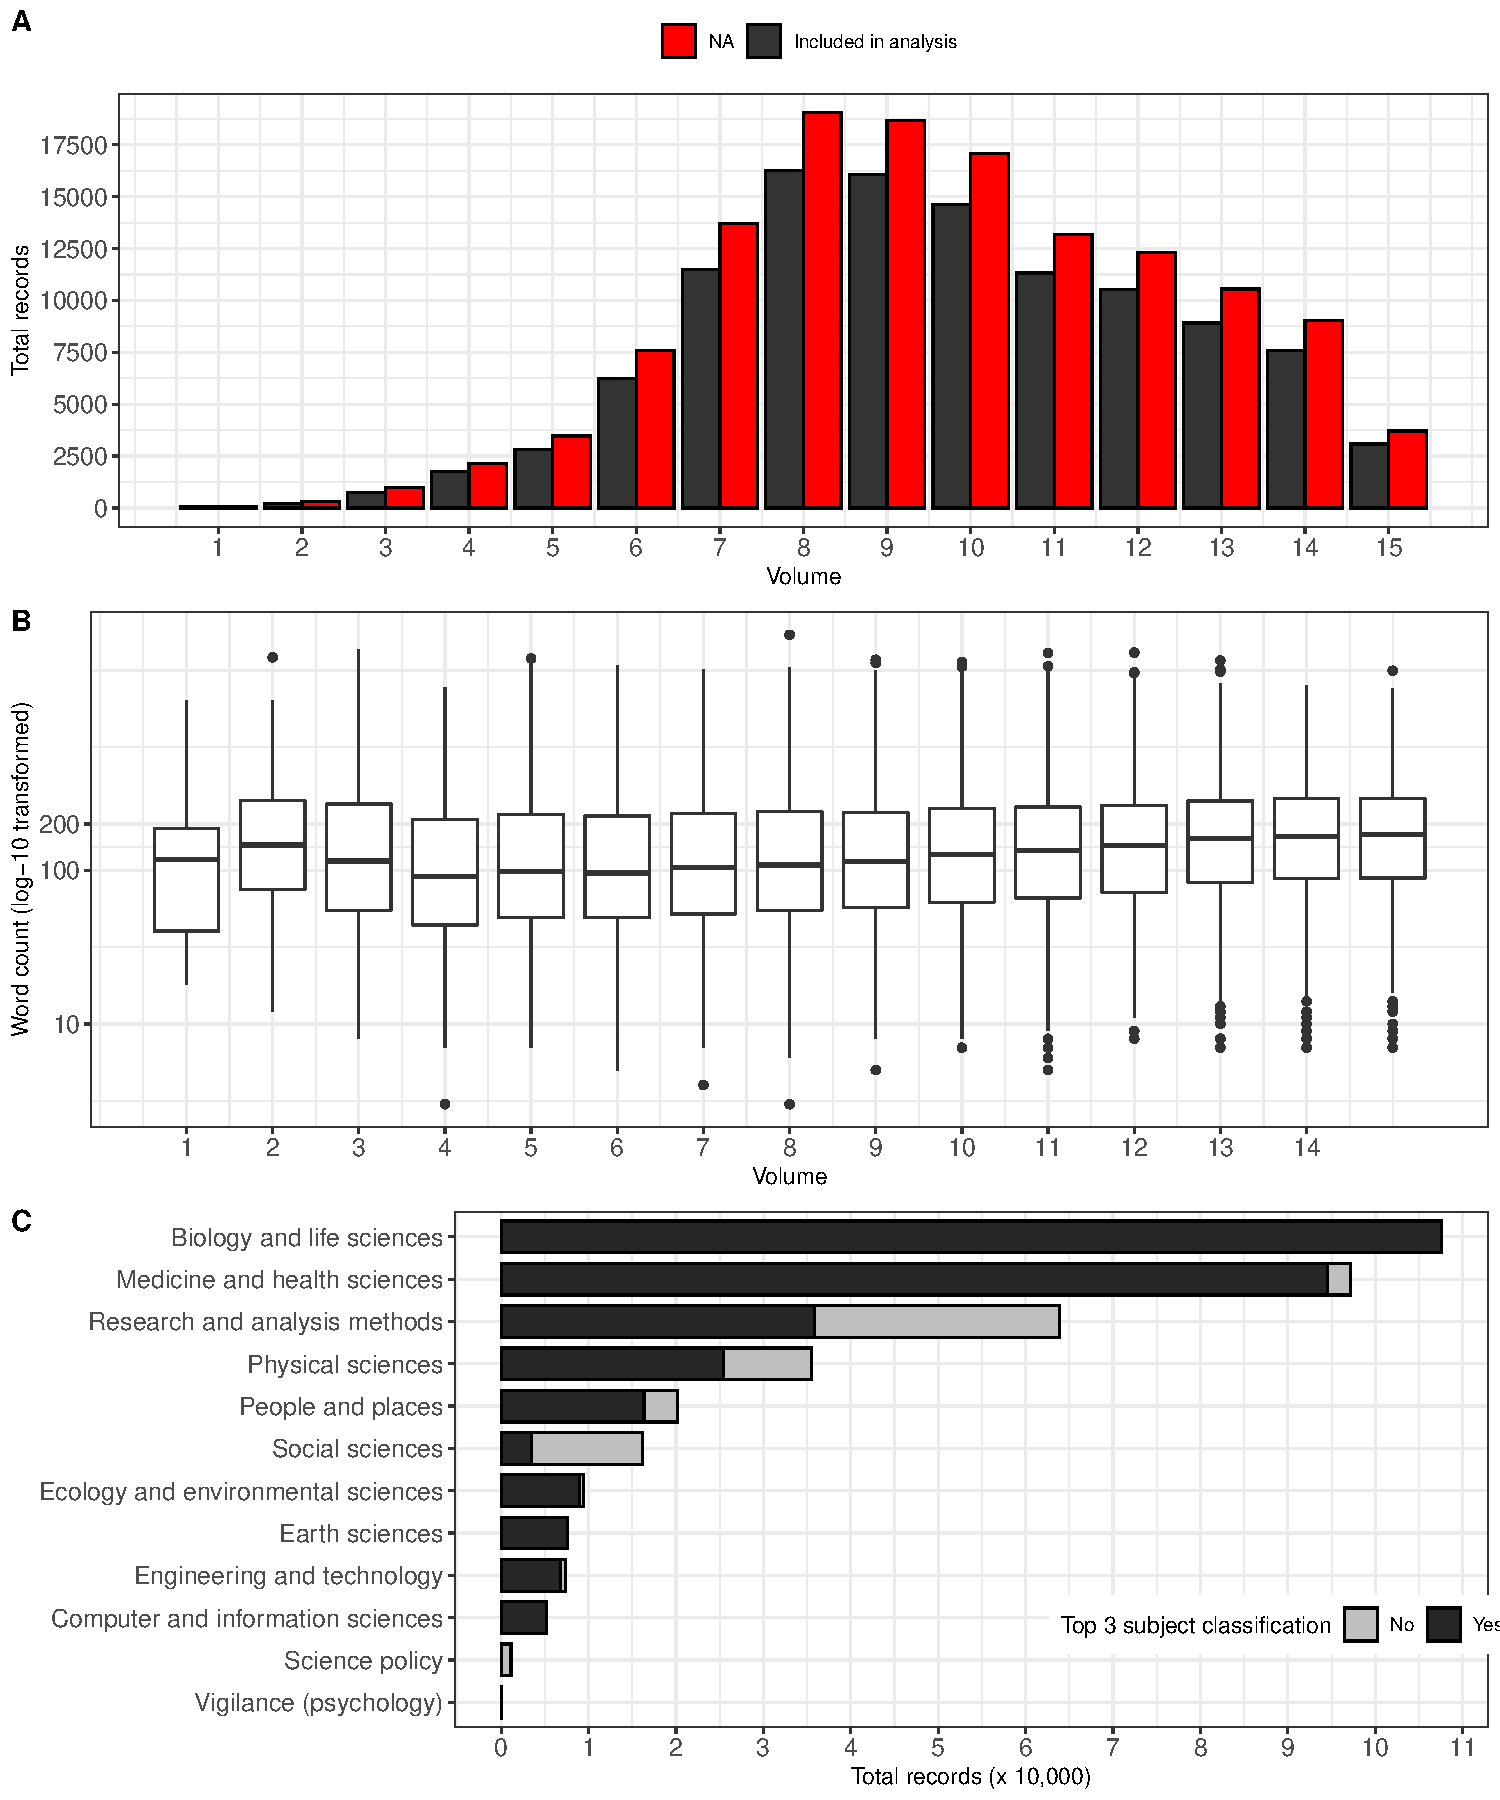
\includegraphics{draft_manuscript_files/figure-latex/unnamed-chunk-3-1.pdf}
\caption{\label{fig:unnamed-chunk-3}\label{fig:plos-n}Search results by \emph{PLOS ONE} volume (1st row); word count per statistical methods section included in analysis (n = 111,731; 2nd row); subject classifications assigned to full-text records included in analysis (3rd row)}
\end{figure}

API searches returned 131,847 unique records, of which 111,731 (85\%) included a statistical methods section based on our search criteria. In the final sample, 95,518 (85\%) DOIs returned an exact match against common section headings, including 64,133 for `statistical analysis', 13,380 for `statistical analyses' and 13,627 for `data analysis'. Among DOIs that did not meet the partial matching criteria, initial search terms appeared in {[}TODO{]}.

Search results varied by journal volume (Figure \ref{fig:plos-n}A). The total number of API search results peaked at volumes 8 (n = 19,045) and 9 (n = 19,045), corresponding to years 2013 and 2014. This trend aligned with the total number of papers published in \emph{PLOS ONE} over the same period. The percentage of records that included a statistical methods section by volume based on our proposed matching criteria varied between 64\% (volume 2) and 86\% (volume 9).

The median length of statistical methods sections was 127 words (IQR: 61 to 253 words) (Figure \ref{fig:plos-n}B). 7,348 articles (7\%) had a statistical methods section of 500 words or more. 19,479 articles (17\%) had a statistical methods section of 50 words or less, equal to the length of this paragraph.

All papers included Biology and life sciences (n = 107,584), Earth sciences
(n = 7,605) and/or Computer and information sciences (n = 5,190) in their top 3 subject classifications
(Figure \ref{fig:plos-n}C).

We applied the clustering algorithm to the cleaned dataset, varying the number of clusters from 1 to 50. Increasing the number of clusters decreased cluster quality based on global goodness-of-fit measures (Supplementary Figure 1), with average silhouette score and within-cluster dispersion leveling off around 20 clusters. This indicated that the data comprised one large, heterogeneous cluster and multiple smaller clusters.

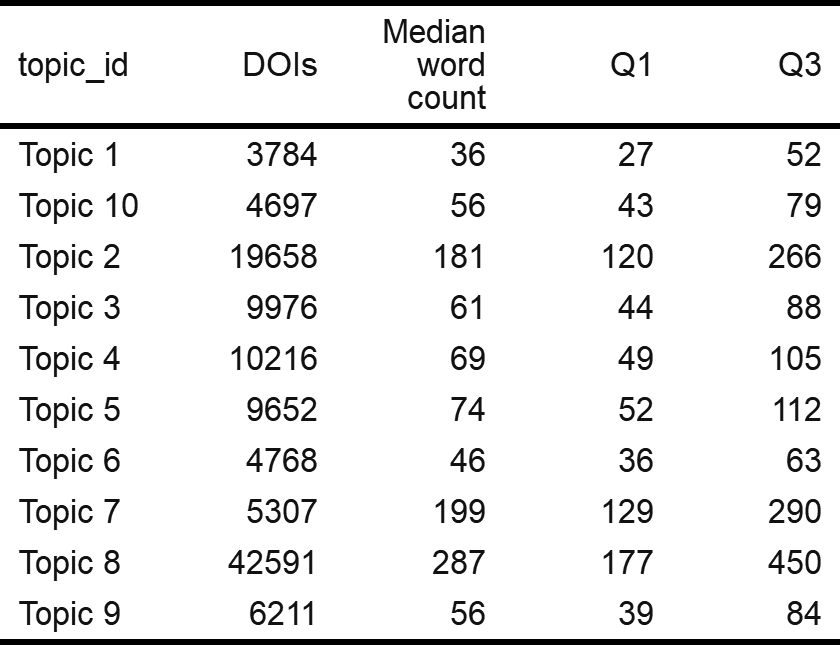
\includegraphics[width=3.75in,height=2.75in,keepaspectratio]{draft_manuscript_files/figure-latex/unnamed-chunk-4-1.png}

The topic clouds based on ten clusters are in Figure\textasciitilde\ref{fig:plot-10-topics}. Frequently occurring words reflected the use of statistical software (Topics\textasciitilde3 and 5), descriptive statistics (Topic\textasciitilde6), group based hypothesis testing (Topics 1 and 4) and definitions of statistical significance (Topics\textasciitilde1 and 9). There are also statistical methods sections associated with regression (Topic\textasciitilde2) and meta-analysis (Topic\textasciitilde7).

Topics related to the use of statistical software differentiated between Prism GraphPad (Topic\textasciitilde3: n = 9,879; 8.8\%) and SPSS (Topic 5: n = 9,574; 8.6\%) (Box 1). A manual review of the top matching sections in these topics showed strong evidence of boilerplate text. Nine out ten top matches for Topic 3 stated the use of Prism GraphPad but did not specify which statistical methods were used; six out of ten top matches returned the same cluster score indicating near identical text. Top matching sections for Topic 5 included information on SPSS version numbers and definitions of statistical significance.

\begin{center}\rule{0.5\linewidth}{0.5pt}\end{center}

\textbf{Box 1: Examples of boilerplate text from \emph{PLOS ONE} (Statistical software)}

Topic 3

\begin{itemize}
\tightlist
\item
  \emph{graphpad prism (graphpad software, san diego, ca) was used for all analyses.}
\item
  \emph{all statistical analysis was performed using the graphpad prism software.}
\item
  \emph{statistical analysis were done using graphpad prism software (graphpad software, inc., la jolla, ca).}
\end{itemize}

Topic 5

\begin{itemize}
\tightlist
\item
  \emph{all statistical analyses were conducted in spss 19 (spss inc., chicago, il, usa).}
\item
  \emph{all statistical analyses were performed using the spss version 15 for windows (spss inc., chicago, il, usa). a p-value less than 0.05 was considered a significant difference.}
\item
  \emph{statistical analysis was performed using the spss 17.0 software package (spss, chicago, il, usa). all data were analyzed using t tests, values of p \textless{} 0.05 were considered significant.}
\end{itemize}

\begin{center}\rule{0.5\linewidth}{0.5pt}\end{center}

Definitions of statistical significance featured strongly in Topic\textasciitilde1 (n = 3,775) and Topic 9 (n = 6,104) combined with hypothesis testing for comparing differences between two groups. Topic\textasciitilde1 reflected applications of Student's t-test assuming a 5\% level of statistical significance. Topic\textasciitilde9 referenced similar methods combined with multiple thresholds for declaring statistical significance by asterisk: ``*p\textless0.05, **p\textless0.01 and ***p\textless0.001'', a practice that has been criticised (Wasserstein, Schirm, and Lazar \protect\hyperlink{ref-Wasserstein2019}{2019}). Examples of boilerplate text are in Box\textasciitilde2.

\begin{center}\rule{0.5\linewidth}{0.5pt}\end{center}

\textbf{Box 2: Examples of boilerplate text from \emph{PLOS ONE} (Between-group hypothesis testing, two groups)}

Topic 1

\begin{itemize}
\tightlist
\item
  \emph{student's t-test was used for statistical analysis. a p value of \textless0.05 was considered statistically significant.}
\item
  \emph{statistical analysis was performed using student`s t-test. a p-value \textless0.05 was considered to be statistically significant.}
\item
  \emph{statistical analysis was performed using a two-tailed student's t-test, and p-values \textless0.05 were considered statistically significant.}
\end{itemize}

Topic 9

\begin{itemize}
\tightlist
\item
  \emph{statistical significance was determined by students t-tests. * p\textless0.05, ** p = \textless0.01, *** p\textless0.001.}
\item
  \emph{statistical analyses were performed using the nonparametric mann-whitney test. differences were considered significant for} *\emph{p\textless0.05,} ** \emph{p\textless0.01, *** }p\textless0.001.*
\item
  \emph{comparisons between two groups were performed by student's test. statistical significance was defined as *}p\textless0.05;* ** \emph{p\textless0.01;} *** \emph{p\textless0.001.}
\end{itemize}

\begin{center}\rule{0.5\linewidth}{0.5pt}\end{center}

Group-based hypothesis testing was a recurring theme across topics, with text descriptions varying based on method(s) used (Box 3). Frequently occurring words in Topic 6 (n = 4,746) including `mean', `sd' and `sem' reflected the use of descriptive statistics for summarising continuous variables. Sections associated with this topic appeared to be expanded versions of Topics 1 and 9, showing evidence of boilerplate text in the form of descriptive statistics followed by hypothesis testing using Student's t-test, Mann Whitney U or one-way analysis of variance. One-way analysis of variance also featured strongly in Topic 4 (n = 10,163), with text citing common methods for performing post-hoc multiple comparisons. Top matching sections across these topics did not include definitions of groups being compared.

\begin{center}\rule{0.5\linewidth}{0.5pt}\end{center}

\textbf{Box 3: Examples of boilerplate text from \emph{PLOS ONE} (Between-group hypothesis testing, two or more groups)}

Topic 4

\begin{itemize}
\tightlist
\item
  \emph{significant differences were determined using analysis-of-variance anova followed by tukey post-hoc tests for multiple comparisons.}
\item
  \emph{statistical comparisons between study groups were performed using one-way anova test followed by post-hoc multiple comparison with dunnett test. p-value of less-than 0.05 were considered to be statistically significant.}
\item
  \emph{one-way analysis-of-variance anova was used to compare multiple groups followed by bonferroni post-hoc test. statistical significance was set at p less-than 0.05.}
\end{itemize}

Topic 6

\begin{itemize}
\tightlist
\item
  \emph{all results are expressed as means plus-or-minus standard deviation plus-or-minus sd.}
\item
  \emph{data are presented as mean plus-or-minus sd or mean plus-or-minus sem. comparison of means was performed by anova test.}
\item
  \emph{data are expressed as means plus-or-minus standard error of the mean sem. statistical analysis was performed using the student t-test. p less-than 0.05 was considered significant.}
\end{itemize}

\begin{center}\rule{0.5\linewidth}{0.5pt}\end{center}

\hypertarget{anzctr}{%
\subsection{ANZCTR}\label{anzctr}}

We downloaded 28,008 studies. The numbers of excluded studies are shown in Figure\textasciitilde X.
Of the 12,700 included studies, 9,523 (75\%) had a statistical methods section.

The median length of the section was 129 words with an inter-quartile range of 71 to 219 words.
Some methods sections were only one word, including ``ANOVA'', ``t-test'', ``SPSS'' and even ``SSPS''.

The clustering algorithm found groups that were purely sample size calculations (topic 2), pilot studies (topic 5), safety/tolerability studies (topic 6) and repeated measures ANOVA (topic 10). There were cases where the exact same method section had been re-used in a different study.

We also found evidence of `boilerplate' sections clustered as topic 3, example text

\begin{center}\rule{0.5\linewidth}{0.5pt}\end{center}

\textbf{Box x: Examples of boilerplate text from ANZCTR}

Topic 3

\begin{itemize}
\tightlist
\item
  ``Shapiro Wilk test was used as normality test. Continuous variables were compared using Student t-test and Mann-Whitney U test when the data were not normally distributed. Categorical variables were compared using Pearson's chi-squared test and Fisher's exact test. Paired data were analyzed using Paired t-test and Wilcoxon signed rank test when data were not normally distributed.''
\item
  ``Comparisons between categorical variables will be made either using chi square or Fisher exact test. Continuous data will be compared using the Student's t-test or Mann-Whitney U test. Two sided p values of less than 0.05 will be considered statistically significant.''
  \_\_\_
\end{itemize}

We examined if four study characteristics were associated with a missing statistics section. The odds ratios and 95\% credible intervals are in Table\textasciitilde X. Observational studies were less likely to have a missing methods section compared with interventional studies. Missing sections became less likely over time. Studies with more funders and a larger target sample size were less likely to have a missing methods section.

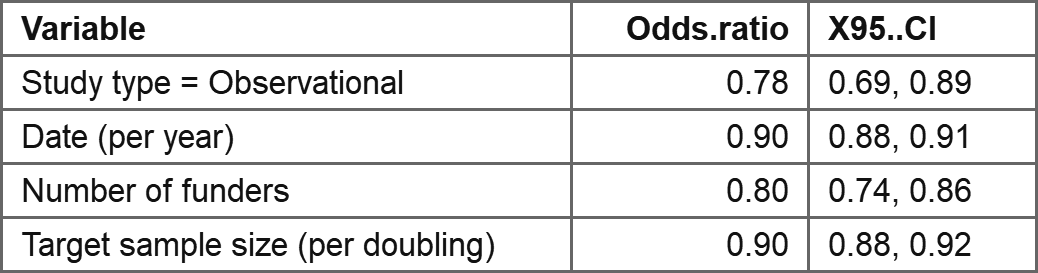
\includegraphics[width=4.66in,height=1.55in,keepaspectratio]{draft_manuscript_files/figure-latex/unnamed-chunk-5-1.png}

\begin{itemize}
\tightlist
\item
  Final sample size
\end{itemize}

\hypertarget{discussion}{%
\section{Discussion}\label{discussion}}

The first line in many statistical analysis sections in \emph{PLOS ONE} was the software used and some entire sections in ANZCTR only stated the software, implying that the software is the most important detail. As Doug Altman said, ``Many people think that all you need to do statistics is a computer and appropriate software'' (Altman \protect\hyperlink{ref-Altman1994}{1994}). This is far from the truth, and whilst it is important for researchers to mention the software and version used for reproducibility purposes, it is a minor detail compared with detailing what methods were used and why.

A frequent theme in the boilerplate statistical methods is the definition of statistical significance, nearly always using a p-value at the 5\% level. This widespread use of statistical significance is troubling giving the bright-line thinking it engenders (McShane et al. \protect\hyperlink{ref-McShane2019}{2019}) and the common misinterpretations of p-values (Goodman \protect\hyperlink{ref-Goodman2008}{2008}).

Despite the extensive array of statistical tests available, many authors are reporting the same few methods.

One reason these inadequate sections get published is that most journals do not use statistical reviewers, despite empirical evidence showing they improve manuscript quality (Hardwicke and Goodman \protect\hyperlink{ref-Hardwicke2020}{2020}).

A related paper has criticised vague statistical methods sections because they deprive readers and reviewers for the opportunity to confirm that the appropriate methods were used (Weissgerber Tracey et al. \protect\hyperlink{ref-Weissgerber2018}{2018}). These authors checked hundreds of papers using ANOVA and found that 95\% did not contain the information needed to determine what type of ANOVA was performed. This lack of information could well be because the authors used a boilerplate statistical methods section that was missing key details.

If authors shared their code then this would provide an alternative route for checking what statistical methods were used. This is not a perfect solution, as we still want authors to accurately report their methods, but it does increase transparency. However, a recent paper found that code sharing was very low in biomedical papers, with just 2\% of a sample of over 6,000 papers sharing code (Serghiou \protect\hyperlink{ref-Serghiou2021}{2021}).

Many researchers are using lazy practice by copying a standard ``boilerplate'' statistical methods section, likely cut-and-pasting from other researchers or projects. This is a strong sign of the ritualistic practice of statistics where researchers go through the motions rather than using conscientious practice (Stark and Saltelli \protect\hyperlink{ref-Stark2018}{2018}). This is concerning because using the wrong statistical methods can reduce the value of study, or worse, invalidate the entire study. These mistakes are avoidable and are wasting of thousands of hours of researchers' time and the time of patients and volunteers. Poor statistical practice is a key driver of the ongoing reproducibility crisis in science (Ioannidis et al. \protect\hyperlink{ref-Ioannidis2014}{2014}).

\hypertarget{limitations}{%
\subsection{Limitations}\label{limitations}}

We did not check whether papers used the correct methods, and for some simple studies a `boilerplate' statistical methods might be adequate.

We examined papers where there was a statistics section, and we missed papers that used statistical analysis but did not include a statistical analysis section. Reiterate outcomes of random sample checking here.

We only examined one large journal and one trial registry and hence our results may not be generalisable to all journals or registries, especially those that consistently use a statistical reviewer.

We searched the full text of \emph{PLOS ONE} papers but not the supporting information which may contain statistical methods sections for some papers. The search terms we used to find statistical methods appeared in the supporting information titles for xxx papers (x\%). We did not include the supporting information because it is less structured than the paper and could be in PDF or Word format.

\hypertarget{references}{%
\section*{References}\label{references}}
\addcontentsline{toc}{section}{References}

\hypertarget{refs}{}
\leavevmode\hypertarget{ref-Allison2016}{}%
Allison, David B., Andrew W. Brown, Brandon J. George, and Kathryn A. Kaiser. 2016. ``Reproducibility: A Tragedy of Errors.'' \emph{Nature} 530 (7588): 27--29. \url{https://doi.org/10.1038/530027a}.

\leavevmode\hypertarget{ref-Altman1994}{}%
Altman, D G. 1994. ``The Scandal of Poor Medical Research.'' \emph{BMJ} 308 (6924): 283--84. \url{https://doi.org/10.1136/bmj.308.6924.283}.

\leavevmode\hypertarget{ref-Altman2016}{}%
Altman, Douglas G, and Iveta Simera. 2016. ``A History of the Evolution of Guidelines for Reporting Medical Research: The Long Road to the EQUATOR Network.'' \emph{Journal of the Royal Society of Medicine} 109 (2): 67--77. \url{https://doi.org/10.1177/0141076815625599}.

\leavevmode\hypertarget{ref-ANZCTR}{}%
ANZCTR. 2019. ``ANZCTR Data Field Definitions V25.'' \url{https://www.anzctr.org.au/docs/ANZCTR\%20Data\%20field\%20explanation.pdf}.

\leavevmode\hypertarget{ref-Bland2015}{}%
Bland, M. 2015. \emph{An Introduction to Medical Statistics}. Oxford Medical Publications. Oxford University Press.

\leavevmode\hypertarget{ref-Brown2018}{}%
Brown, Andrew W., Kathryn A. Kaiser, and David B. Allison. 2018. ``Issues with Data and Analyses: Errors, Underlying Themes, and Potential Solutions.'' \emph{Proceedings of the National Academy of Sciences} 115 (11): 2563--70. \url{https://doi.org/10.1073/pnas.1708279115}.

\leavevmode\hypertarget{ref-rplos}{}%
Chamberlain, Scott, Carl Boettiger, and Karthik Ram. 2020. \emph{Rplos: Interface to the Search API for 'PLoS' Journals}. \url{https://CRAN.R-project.org/package=rplos}.

\leavevmode\hypertarget{ref-Diggle2013}{}%
Diggle, P., P. Heagerty, K. Y. Liang, and S. Zeger. 2013. \emph{Analysis of Longitudinal Data}. Oxford Statistical Science Series. OUP Oxford.

\leavevmode\hypertarget{ref-Dobson2018}{}%
Dobson, A. J., and A. G. Barnett. 2018. \emph{An Introduction to Generalized Linear Models}. Chapman \& Hall/Crc Texts in Statistical Science. CRC Press.

\leavevmode\hypertarget{ref-Ernst2017}{}%
Ernst, Anja F., and Casper J. Albers. 2017. ``Regression Assumptions in Clinical Psychology Research Practicea Systematic Review of Common Misconceptions.'' \emph{PeerJ} 5: e3323. \url{https://doi.org/10.7717/peerj.3323}.

\leavevmode\hypertarget{ref-Goodman2008}{}%
Goodman, Steven. 2008. ``A Dirty Dozen: Twelve P-Value Misconceptions.'' \emph{Seminars in Hematology} 45 (3): 135--40. \url{https://doi.org/10.1053/j.seminhematol.2008.04.003}.

\leavevmode\hypertarget{ref-Goodman1998}{}%
Goodman, Steven N., Douglas G. Altman, and Stephen L. George. 1998. ``Statistical Reviewing Policies of Medical Journals.'' \emph{Journal of General Internal Medicine} 13 (11): 753--56. \url{https://doi.org/10.1046/j.1525-1497.1998.00227.x}.

\leavevmode\hypertarget{ref-Hardwicke2020}{}%
Hardwicke, Tom E, and Steve Goodman. 2020. ``How Often Do Leading Biomedical Journalsuse Statistical Experts to Evaluate Statistical Methods? The Results of a Survey.'' MetaArXiv. \url{https://doi.org/10.31222/osf.io/z27u4}.

\leavevmode\hypertarget{ref-ICMJE2019}{}%
ICJME. 2019. ``Recommendations for the Conduct, Reporting, Editing, and Publication of Scholarly Work in Medical Journals.'' \url{http://www.icmje.org/icmje-recommendations.pdf}.

\leavevmode\hypertarget{ref-Ioannidis2014}{}%
Ioannidis, John P A, Sander Greenland, Mark A Hlatky, Muin J Khoury, Malcolm R Macleod, David Moher, Kenneth F Schulz, and Robert Tibshirani. 2014. ``Increasing Value and Reducing Waste in Research Design, Conduct, and Analysis.'' \emph{The Lancet} 383 (9912): 166--75. \url{https://doi.org/10.1016/s0140-6736(13)62227-8}.

\leavevmode\hypertarget{ref-King2019}{}%
King, Kevin M., Michael D. Pullmann, Aaron R. Lyon, Shannon Dorsey, and Cara C. Lewis. 2019. ``Using Implementation Science to Close the Gap Between the Optimal and Typical Practice of Quantitative Methods in Clinical Science.'' \emph{Journal of Abnormal Psychology} 128 (6): 547--62. \url{https://doi.org/10.1037/abn0000417}.

\leavevmode\hypertarget{ref-Lang2013}{}%
Lang, T, and D Altman. 2013. ``Basic Statistical Reporting for Articles Published in Clinical Medical Journals: The SAMPL Guidelines.'' In \emph{Science Editors' Handbook}, edited by P Smart, H Maisonneuve, and A Polderman. European Association of Science Editors.

\leavevmode\hypertarget{ref-Leek2017}{}%
Leek, Jeff, Blakeley B. McShane, Andrew Gelman, David Colquhoun, Michèle B. Nuijten, and Steven N. Goodman. 2017. ``Five Ways to Fix Statistics.'' \emph{Nature} 551 (7682): 557--59. \url{https://doi.org/10.1038/d41586-017-07522-z}.

\leavevmode\hypertarget{ref-McShane2019}{}%
McShane, Blakeley B., David Gal, Andrew Gelman, Christian Robert, and Jennifer L. Tackett. 2019. ``Abandon Statistical Significance.'' \emph{The American Statistician} 73 (sup1): 235--45. \url{https://doi.org/10.1080/00031305.2018.1527253}.

\leavevmode\hypertarget{ref-PLOS}{}%
PLOS. 2021. ``PLOS One: Accelerating the Publication of Peer-Reviewed Science.'' \url{https://journals.plos.org/plosone/s/criteria-for-publication}.

\leavevmode\hypertarget{ref-textclean}{}%
Rinker, Tyler W. 2018. \emph{textclean: Text Cleaning Tools}. Buffalo, New York. \url{https://github.com/trinker/textclean}.

\leavevmode\hypertarget{ref-Serghiou2021}{}%
Serghiou, Despina G. AND Boyack, Stylianos AND Contopoulos-Ioannidis. 2021. ``Assessment of Transparency Indicators Across the Biomedical Literature: How Open Is Open?'' \emph{PLOS Biology} 19 (3): 1--26. \url{https://doi.org/10.1371/journal.pbio.3001107}.

\leavevmode\hypertarget{ref-Stark2018}{}%
Stark, Philip B., and Andrea Saltelli. 2018. ``Cargo-Cult Statistics and Scientific Crisis.'' \emph{Significance} 15 (4): 40--43. \url{https://doi.org/10.1111/j.1740-9713.2018.01174.x}.

\leavevmode\hypertarget{ref-Wasserstein2019}{}%
Wasserstein, Ronald L., Allen L. Schirm, and Nicole A. Lazar. 2019. ``Moving to a World Beyond ``P0.167em\(\less\)0.167em0.05''.'' \emph{The American Statistician} 73 (sup1): 1--19. \url{https://doi.org/10.1080/00031305.2019.1583913}.

\leavevmode\hypertarget{ref-Weissgerber2018}{}%
Weissgerber Tracey, L., Oscar Garcia-Valencia, Vesna D. Garovic, Natasa M. Milic, and Stacey J. Winham. 2018. ``Why We Need to Report More Than 'Data Were Analyzed by T-Tests or ANOVA'.'' \emph{eLife} 7. \url{https://gateway.library.qut.edu.au/login?url=https://search.proquest.com/docview/2174217344?accountid=13380}.

\leavevmode\hypertarget{ref-Wikipedia}{}%
Wikipedia. 2021. ``Boilerplate Text.'' \url{https://en.wikipedia.org/wiki/Boilerplate_text}.

\leavevmode\hypertarget{ref-Zhou2018}{}%
Zhou, Yuanyuan, and Susan Skidmore. 2018. ``A Reassessment of ANOVA Reporting Practices: A Review of Three APA Journals.'' \emph{Journal of Methods and Measurement in the Social Sciences} 8 (1): 3--19. \url{https://doi.org/10.2458/v8i1.22019}.

\end{document}
